\section{Theorie}
\label{sec:Theorie}
\subsection{Wechselwirkung von Gammastrahlung mit Materie}
Die Wechselwirkung von hochenergetischen Photonen aus der Gammastrahlung lässt sich auf 3 zentrale Prozesse reduzieren: den Photoeffekt, den Comptoneffekt und die Paarbildung.
In Abbildung \ref{fig:Wechselwirkung} sind die Prozesse schematisch dargestellt.
\begin{figure}[H]
    \centering
    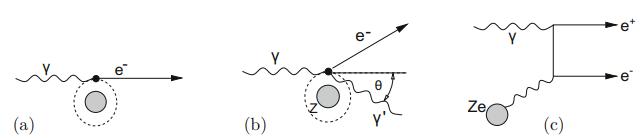
\includegraphics[scale=1.0]{illustration/WWPhoton.png}
    \caption{a) Photoeffekt b) Comptoneffekt c) Paarbildung.\cite{Detektor}}
    \label{fig:Wechselwirkung}
\end{figure}
\noindent Beim Photoeffekt wird das Photon von einem Hüllenelektron vollständig absorbiert und gibt dabei seine gesamte Energie an das Elektron ab. Das Elektron wird dabei aus der Atomhülle gelöst und es entsteht ein freier Platz in der Hülle, 
wenn das Photon genug Energie besitzt, um das Elektron aus der Atomhülle zu lösen. Die Energie des Photons muss dabei mindestens so groß sein wie die Bindungsenergie des Elektrons.
Dies ist bei Photonen der Gammastrahlung der Fall. Dies ist ein Absorptionsprozess. Aufgrund der diskreten Energien der Photonen der Gammastrahlung, der dagegen vernachlässigbaren Bandlücke des Germaniumhalbeiters und 
der Tatsache, dass ein Elektron die volle Energie absorbiert, kann angenommen werden, dass die detektierte Energie dieses Elektron der gesamten 
Energie des Photons entspricht.

\noindent Der Comptoneffekt ist ein Streuprozess, bei dem das Photon an einem freien Elektron gestreut wird. Dabei gibt das Photon einen Teil seiner Energie an das Elektron ab und wird in einem Winkel $\theta$ gestreut.
Das Photon selbst existiert also weiter nach dem Stoß und das Elektron nimmt daher nur einen Teil der Photonenenergie auf. Gemäß der Formel 
\begin{equation}
    \label{eq:Compton}
    E' = \frac{E}{1+\frac{E}{m_0c^2}(1-\cos(\theta))}
\end{equation}
wird die Photonenenergie $E'$ minimal bei Rückstreuung. Daher definiert dieser Punkt die sogenannte Comptonkante, die die maximale Energie der detektierten Elektronen 
definiert, die beim Comptoneffekt beteiligt sind. Der differentielle Wirkungsquerschnitt gibt die Wahrscheinlichkeit an, für eine Streuung in einen bestimmten Raumwinkel.
Für den Comptoneffekt ist dieser Wirkungsquerschnitt gegeben durch die Klein-Nishina-Formel
\begin{equation}
    \label{eq:KleinNishina}
    \frac{d\sigma}{d\Omega} = \frac{r_e^2}{2[1+\epsilon(1-\cos(\theta))]^2}\left(1+cos^2(\theta)+\frac{\epsilon^2(1-\cos(\theta))^2}{1+\epsilon(1-\cos(\theta))}\right)
\end{equation}
mit $\epsilon=\frac{E}{m_0c^2}$ und dem klassischen Elektronenradius $r_e$. In Abbildung \ref{fig:Photo} ist der Wirkungsquerschnitt in Abhängigkeit vom Streuwinkel $\theta$ dargestellt.
In $\phi$-Richtung ist der Wirkungsquerschnitt konstant.
\begin{figure}[H]
    \centering
    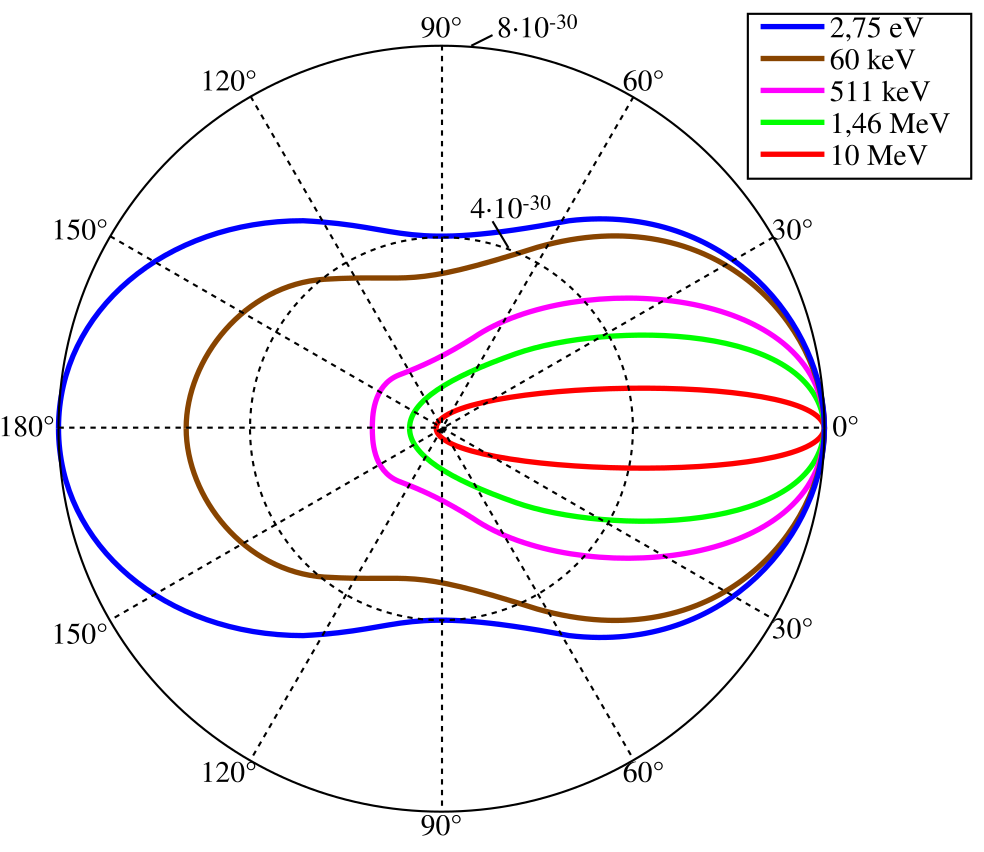
\includegraphics[scale=0.3]{illustration/Klein-Nishina_distribution-en.svg.png}
    \caption{Wirkungsquerschnitt bei Streuung von Photonen an einem Elektron (Compton-Streuung).\cite {Klein}}
    \label{fig:Photo}
\end{figure}

\noindent Die Paarbildung ist ein Prozess, bei dem das Photon in der Nähe eines Atomkerns in ein Elektron-Positron-Paar umgewandelt wird. Dabei muss die Energie des Photons mindestens doppelt so groß sein wie die Ruhemasse des Elektrons.
zusätzlich kann dieser Prozess nur in der Nähe eines Atomkerns stattfinden, da der Impuls des Photons erhalten bleiben muss. Dieser Prozess wird erst bei Photonenenergien deutlich über $1\si{\mega\electronvolt}$ relevant.
Solch hohen Energien werden in diesem Versuch nicht detektiert.

\noindent In Abbildung \ref{fig:Extinktion} ist der Extinktionskoeffizient $\epsilon$ von Germanium in Abhängigkeit von der Energie der Gammastrahlung und der Art der Wechselwirkung dargestellt.
Er gibt an wie stark die Intensität der Gammastrahlung pro Wegstrecke mit $ I(z)=I_0\exp(-\epsilon z)$ abnimmt.
\begin{figure}[H]
    \centering
    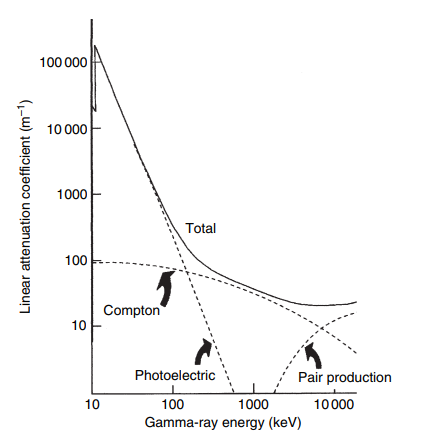
\includegraphics[scale=1.0]{illustration/Extinktionskoeffizient.png}
    \caption{Extinktionskoeffizient von Germanium in Abhängigkeit von der Energie der Gammastrahlung und der Art der Wechselwirkung.\cite{GammaRay}}
    \label{fig:Extinktion}
\end{figure}
\noindent Bei Energien zwischen $100\si{\kilo\electronvolt}$ und $2\si{\mega\electronvolt}$ dominiert der Comptoneffekt, wobei auch der Photoeffekt noch als Vollenergienachweis genutzt werden kann.
Die Interaktionswahrscheinlichkeit steigt beim Comptoneffekt linear mit der Kernladungszahl $Z$ des Absorbermaterials an, während sie beim Photoeffekt quadratisch mit $Z$ ansteigt.
Germanium hat eine relativ hohe Kernladungszahl von $Z=32$, weshalb auch noch viele Photonen über den Photoeffekt detektiert werden können, welcher auf Grund der diskreten 
Energie der Elektronen das Spektrum der Probe am besten charakterisiert. 
\subsection{Gammaspektren}
-chrakteristische Linien
\begin{figure}[H]
    \centering
    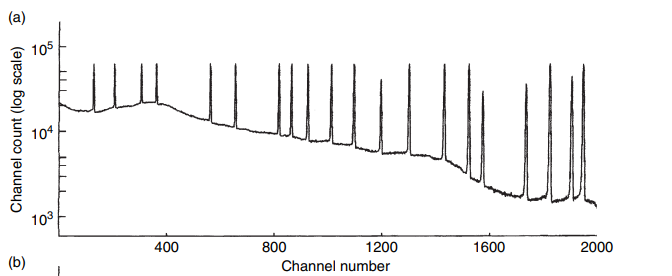
\includegraphics[scale=1.0]{illustration/LinienSpektrum.png}
    \caption{Beispiel eines Gammaspektrums mit charakteristischen Linien.\cite{GammaRay}}
    \label{fig:Spektrum}
\end{figure}
-moochromatisches Spektrum
\begin{figure}{H}
    \centering
    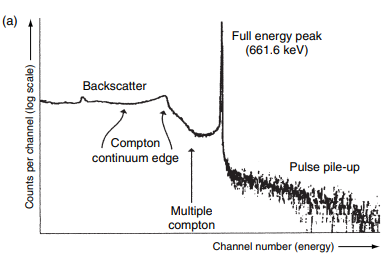
\includegraphics[scale=1.0]{illustration/MonoSpektrum.png}
    \caption{Monochromatisches Gamma-Spektrum.\cite{GammaRay}}
    \label{fig:Mono}
\end{figure}

\subsection{Statistik der Gammapeaks}
-Zählexperimente Poissonverteilt
-Absorptionswahrscheinlichkeit
-Effizienz/Vollenergienachweiswahrscheinlichkeit
\subsection{Halbleitergrundlagen}
-Energiebänder
-direkt/indirekt
-Dotierung
\subsection{Aufbau eines Germaniumdetektors}
-Aufbau/Zonen/Spannung
-Signalentstehung

\subsection{Signalverarbeitung}
-Preamp
-Shaping/Amp
-MCA
\subsection{Unschärfe der Photopeaks}
-Rauschen(Elektronik)
-thermische Übergänge im Detekor
-intrinsische Unschärfe
-unschärfe in Anzahl erzeugter und detektierter Elektronen
-Abschirmung

% \begin{equation}
%     \label{eq:}

% \end{equation}
% \begin{figure}[H]
%     \centering
%     \includegraphics[scale=0.5]{content/}
%     \caption{\cite{}.}
%     \label{fig:}
% \end{figure}

%\cite{}
